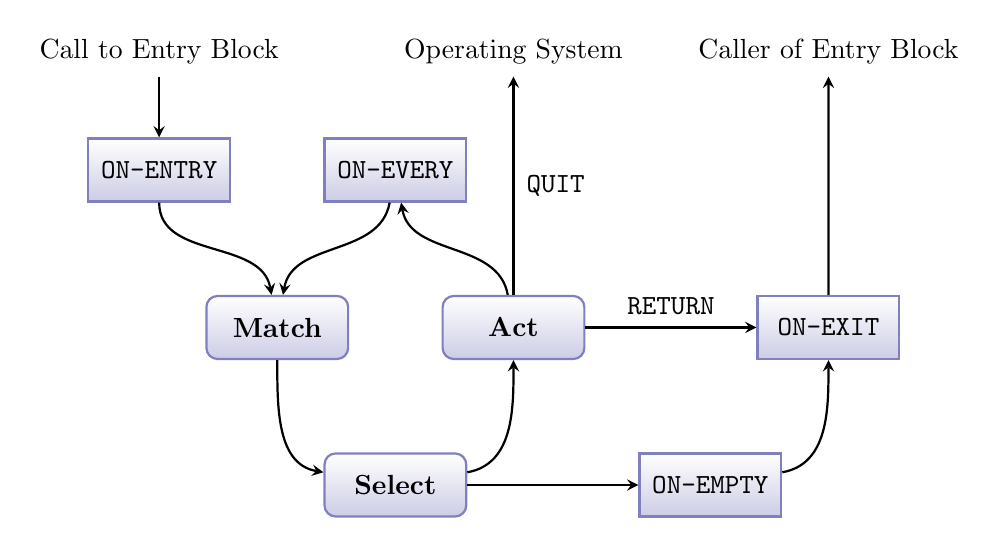
\begin{tikzpicture}[
  node distance=1mm,
  inner sep=1ex,
%  text height=1.7ex,
%  text depth=.25ex,
%  font=\small,
  box/.style={ 
    thick,
    draw=blue!50!black!50,
    top color=white,
    minimum height=0.8cm,
    minimum width=1.8cm,
    bottom color=blue!50!black!20
  },
  rounded corner/.style={
    rounded corners=10pt
  },
  a/.style={
    -stealth,
    thick
  }
  ]

  \node (on-entry) [box] at (0,0) {\texttt{ON-ENTRY}};
  \node (on-every) [box] at (3cm,0) {\texttt{ON-EVERY}};
  \node (match) [box,rounded corners] at (1.5cm,-2cm) {\textbf{Match}};
  \node (select) [box,rounded corners] at (3cm,-4cm) {\textbf{Select}};
  \node (act) [box,rounded corners] at (4.5cm,-2cm) {\textbf{Act}};
  \node (on-exit) [box] at (8.5cm,-2cm) {\texttt{ON-EXIT}};
  \node (on-empty) [box] at (7cm,-4cm) {\texttt{ON-EMPTY}};
  \node (operating-system) at (4.5cm,1.5cm) {Operating System};
  \node (call-to-entry-block) at (0,1.5cm) {Call to Entry Block};
  \node (caller-of-entry-block) at (8.5,1.5cm) {Caller of Entry Block};

  \draw [->,a] (on-entry) to[out=270,in=100] (match);
  \draw [->,a] (on-every) to[out=260,in=80] (match);
  \draw [->,a] (match) to[out=270,in=170] (select);
  \draw [->,a] (select) to[out=10,in=270] (act);
  \draw [->,a] (select) to (on-empty);
  \draw [->,a] (on-empty) to[out=10,in=270] (on-exit);
  \draw [->,a] (act) to[out=100,in=280] (on-every);
  \draw [->,a] (act) to node [midway,above] {\texttt{RETURN}} (on-exit);
  \draw [->,a] (act) to  node[midway,right] {\texttt{QUIT}} (operating-system);
  \draw [->,a] (on-exit) to (caller-of-entry-block);
  \draw [->,a] (call-to-entry-block) to (on-entry);
\end{tikzpicture}

%%% Local Variables:
%%% mode: latex
%%% TeX-master: "rwug"
%%% End:
